This section presents the system architecture of the designed artifact, CodeClusters. While the background research provided various theoretical and practical approaches how to analyze and cluster the submissions to provide feedback, their use was limited to the actual software development process. The majority of development on the system was spent on the UI and the more difficult parts, such as the models and search, were based on the available libraries and applications. Using popular technologies instead of custom implementations were postulated to make the system more maintainable and modular while also providing extensive capabilities that would otherwise be impossible to add in. The design process of the UI was mostly guided by the feedback of the thesis supervisor and the practical insights that emerged from building and using the system.

The system as a whole was developed to the quality of standard of the author of this thesis, which is based on 3 years of working as a part-time software developer in the industry. In practice, this has meant writing readable and robust code that should pass code reviews by peer software engineers. It has also provided a better understanding in designing systems to be as maintainable and well-documented as possible with scripts and written instructions to perform various operations. The system was licensed under MIT license, which is permissive to most modifications\footnote{\url{https://github.com/Aalto-LeTech/CodeClusters}}\footnote{\url{https://github.com/Aalto-LeTech/CodeClustersModeling}}.

\begin{figure}
\centering 
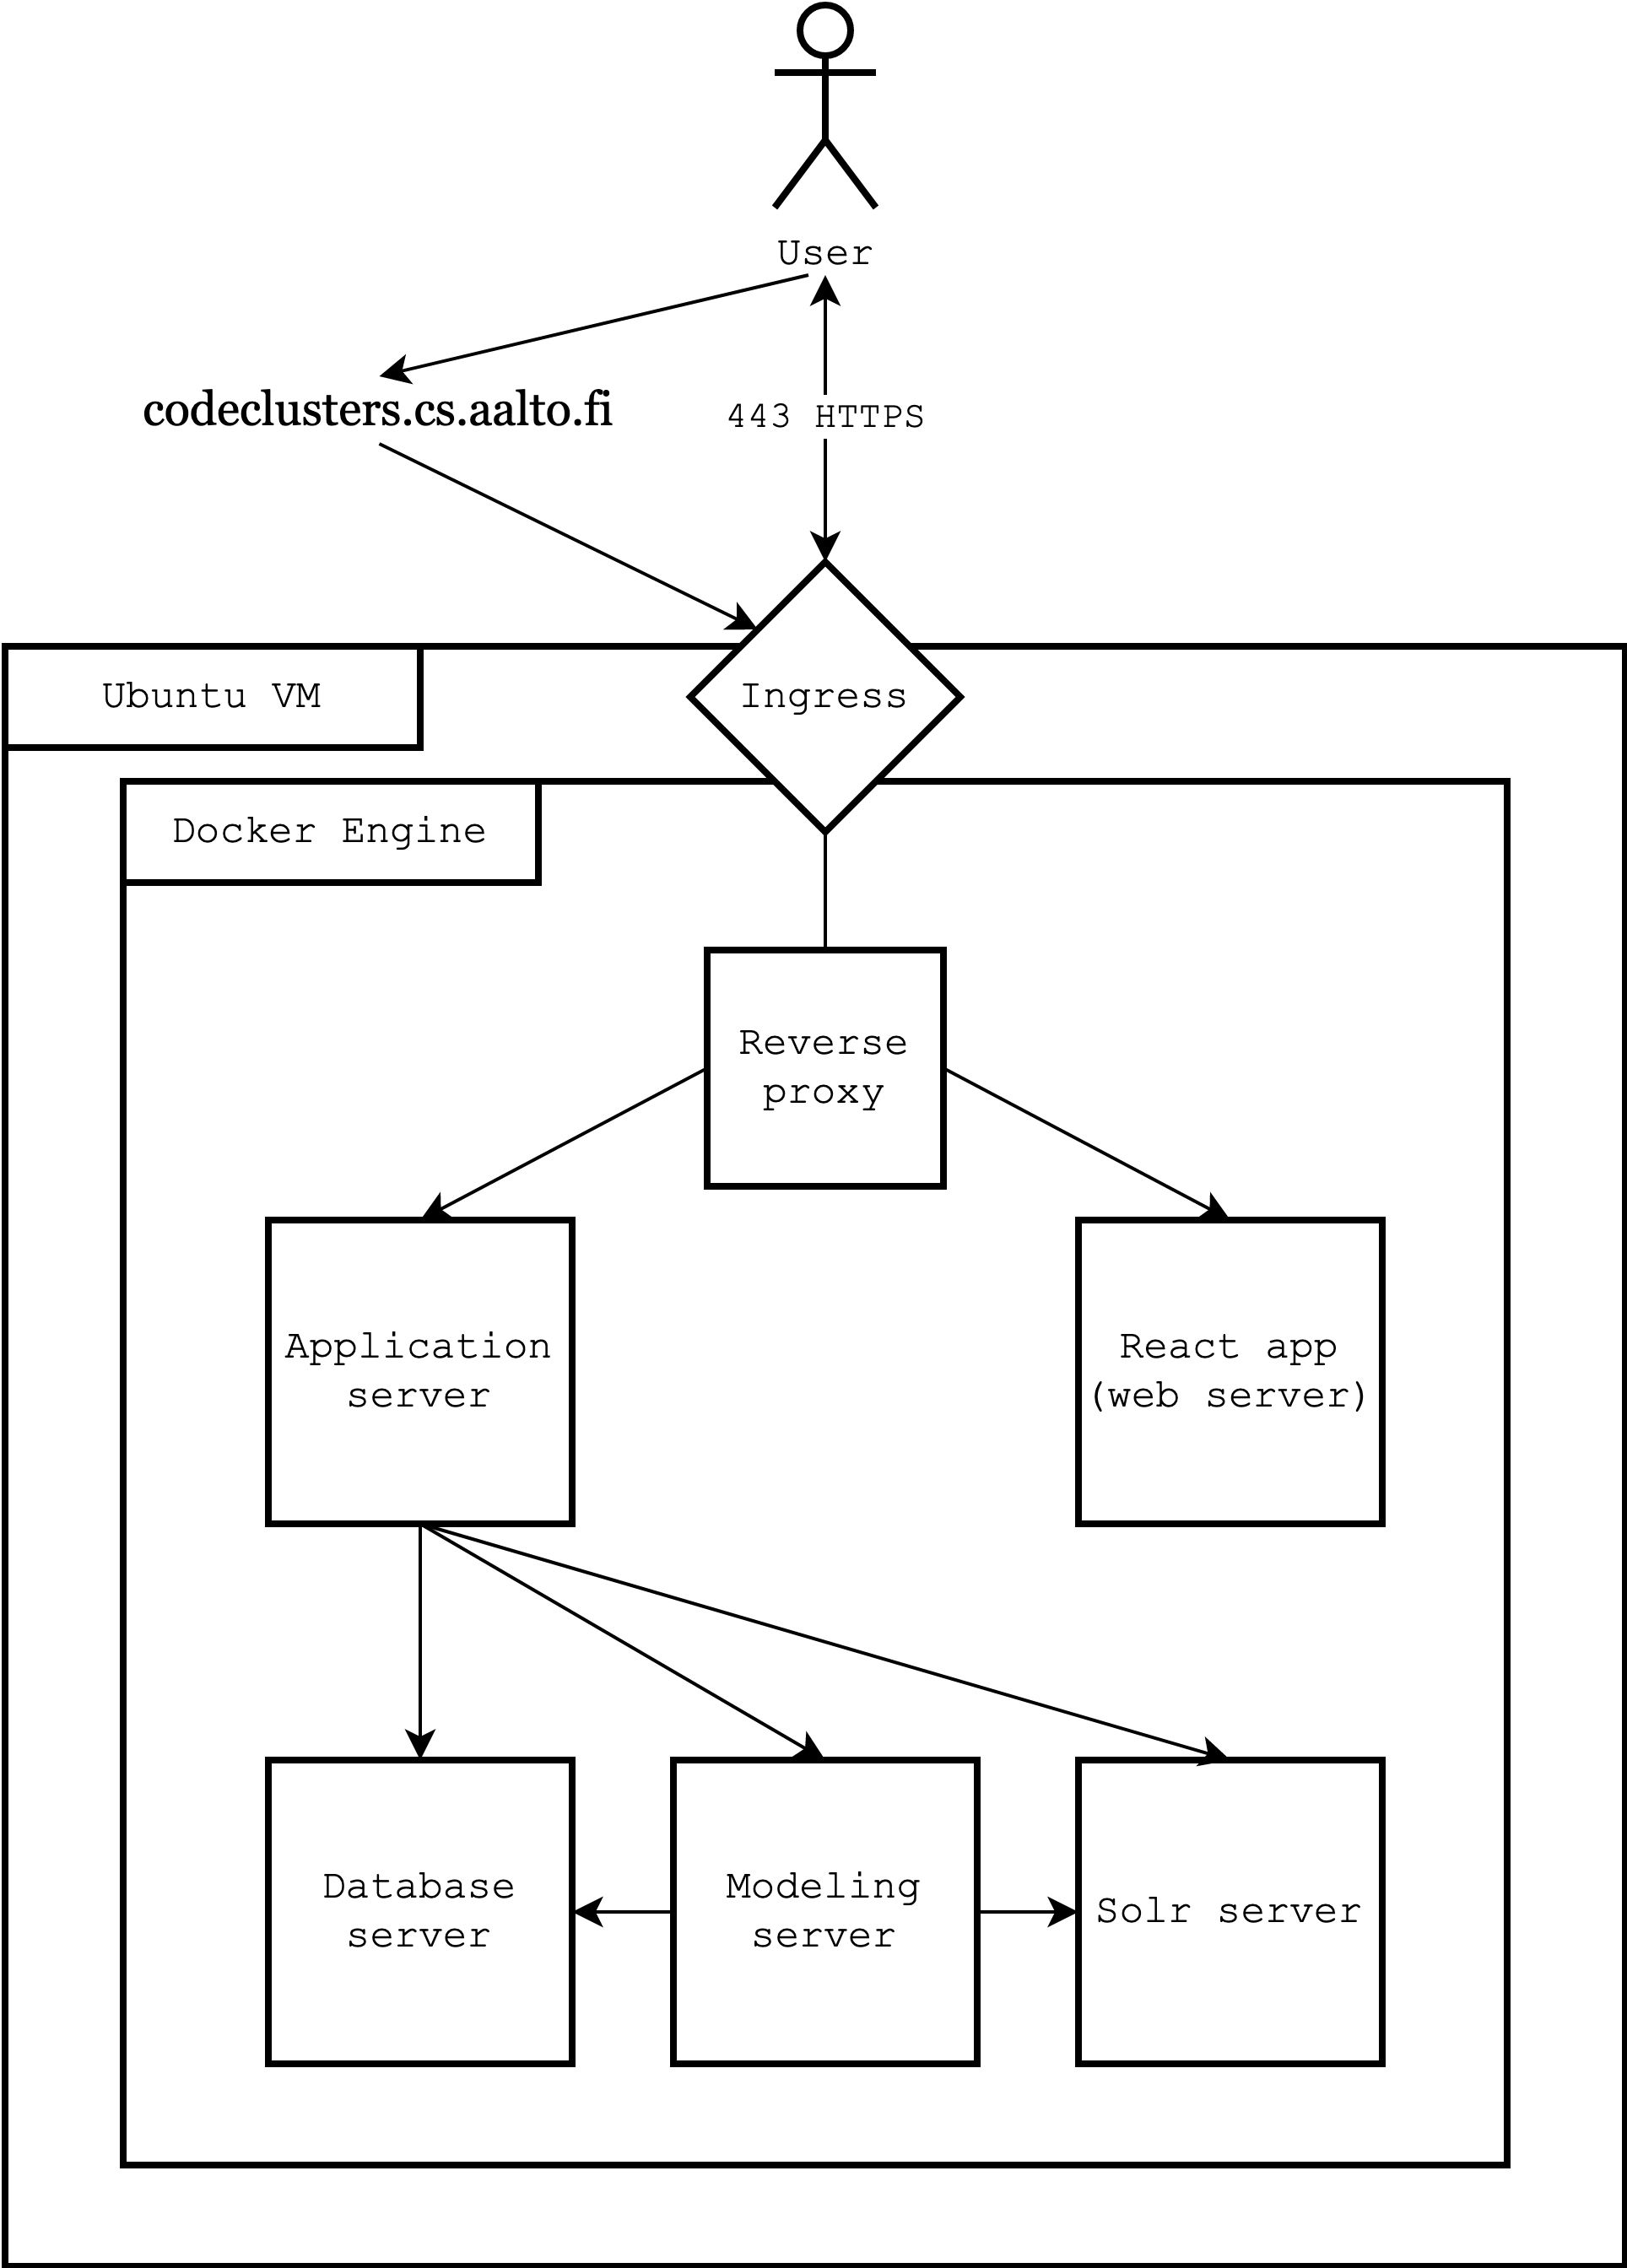
\includegraphics{images/architecture.png}
\caption{Architecture graph of the deployed Docker containers\label{fig:architecture}}
\end{figure}

At its core, CodeClusters is a web site that can be accessed with most web browsers\footnote{\url{https://codeclusters.cs.aalto.fi/}}. It is divided into 6 parts that are run as individual containers on a single Linux Ubuntu virtual machine (VM) (see Fig.~\ref{fig:architecture}). The containers are managed by Docker Compose and the server configuration written as \texttt{docker-compose.yaml} files. This simplifies the development and deployment of the system and using containers allows managing the various dependencies of the servers easily.

Majority of the system is written in TypeScript, with the application server (Node.js\footnote{\url{https://nodejs.org/en/}}) and web application (React\footnote{\url{https://reactjs.org/}}) both written in TypeScript. TypeScript is a popular language in web development that should be fairly easy to learn for anyone familiar with JavaScript. Homogenizing the server and client code enables developers to focus on one particular language, which provides also practical benefits such as sharing code between the two. Perhaps most importantly the author of this system is very familiar with the language, which made it an easy choice. Other used programming languages are HTML, Sass and Python with little snippets of Bash scripts and SQL.

\subsection{Reverse proxy}

The entry point to CodeClusters is the reverse proxy which handles all the incoming requests and forwards them to the correct services. From security standpoint this is important, as single point of entry makes it easy to manage the security and the network configuration of the website, as well as the SSL certificates. It is implemented using Nginx\footnote{\url{https://www.nginx.com/}}, a very popular web server software, due to its good performance and reliability.

\subsection{Web application}

The majority of development effort on CodeClusters was spent on the user interface (see Fig. \ref{fig:cc-frontpage} and Fig. \ref{fig:cc-modeling}), which is a single-page web application (SPA) implemented using the React UI framework. Using a framework such as React helps to organize the UI into modular components that can be composed and reused easily which is a standard practice in web development. React offers a solid structure to the application with most of the difficult parts, mainly re-rendering of the components, abstracted from the developer. It also offers the mixing of different programming languages: HTML, Sass and TypeScript, combined into single \texttt{.tsx} files to keep the code compact. There also exists a large React ecosystem of various libraries which allow the implementation of various complicated UI functionalities with minimal effort. The total amount of code written for the React UI consists of 78 components, 45 other individual files and 10,400 lines of code.

\begin{figure}
\begin{center}
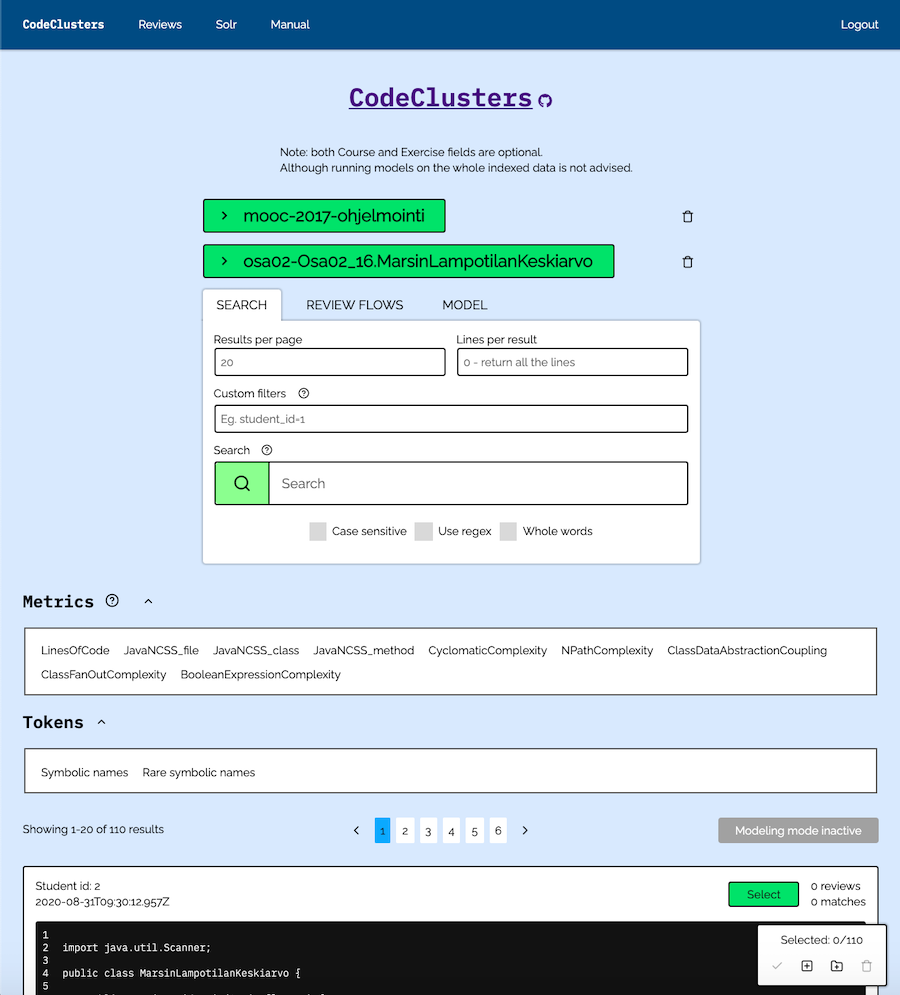
\includegraphics{images/cc-frontpage.png}
\caption{Screenshot of the frontpage of CodeClusters \label{fig:cc-frontpage}}
\end{center}
\end{figure}

The difference between SPAs and regular websites is roughly that SPAs serve the whole site as a single HTML page with the page transitions simulated to the user, whereas regular websites serve individual HTML pages for every URL address. This makes state management of the application easier as the page does not change, and SPAs also reduce the latencies between page loads when navigating the site with the overhead of having the serve the whole application at once. This, however, is a negligible issue with such a small application as CodeClusters.

\begin{figure}
\begin{center}
    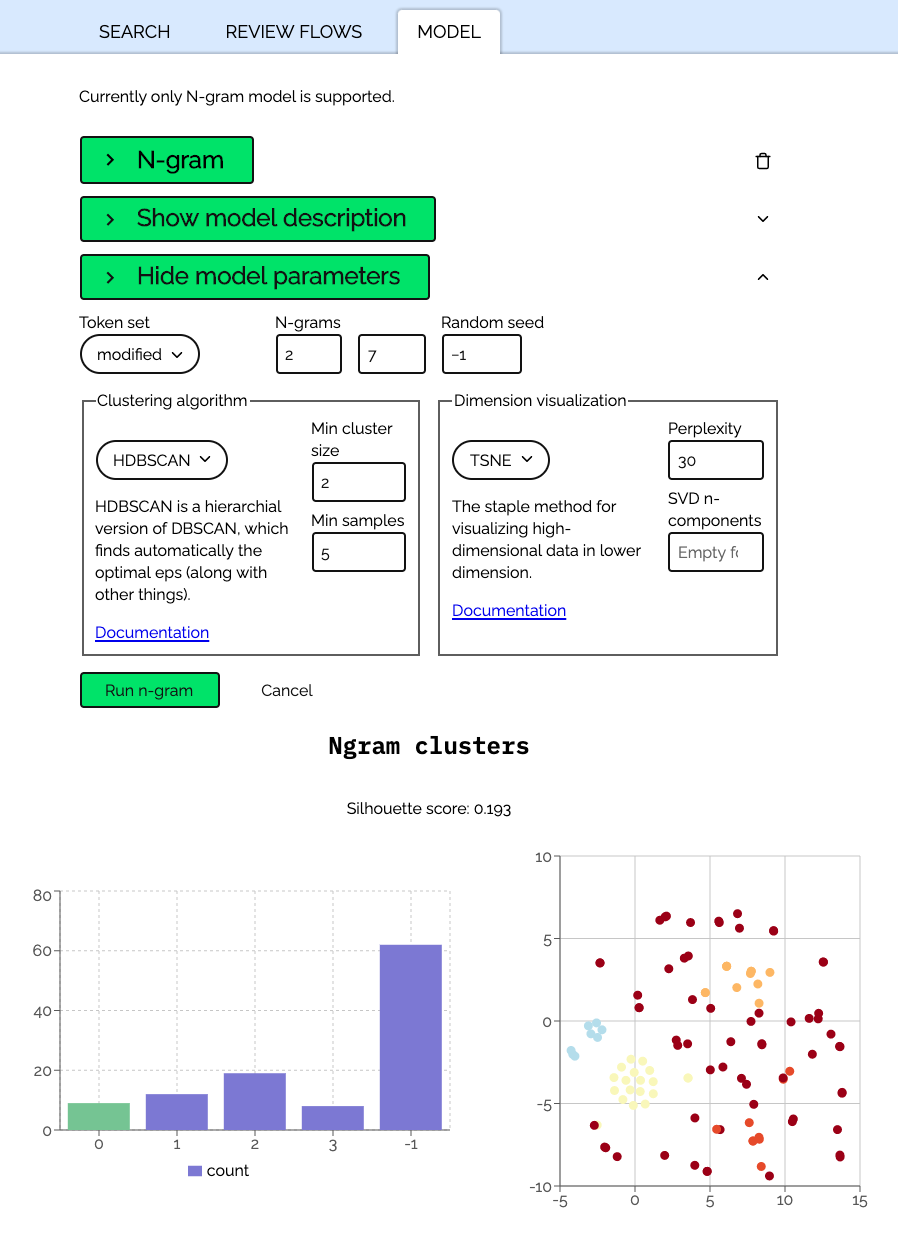
\includegraphics{images/cc-modeling.png}
    \caption{Screenshot of the n-gram model of CodeClusters. The clusters are selectable to allow reviewing of the submissions. \label{fig:cc-modeling}}
\end{center}
\end{figure}

The disadvantages of React are mainly its underlying complexity and design architecture, which requires some expertise to fully leverage and to avoid performance bottlenecks. During the development a few issues with inefficient rendering of components occurred, yet by reorganizing the components and optimizing how they updated the problems were mitigated to large extent. Otherwise, React enjoys a widespread popularity that should make future development on the UI relatively easy.

At the code level, the React code is stored in the same git repository alongside the Node.js server code. This mono-repository simplifies the management of the code between the colloquially called "backend" and "frontend", and also for example the TypeScript type definitions can be easily shared between the two. The React code is further divided into folders of components or functions that share a similar use. They follow the guideline quoted as "kitchenware principle" which means that in the same drawer, comparable to a file directory, you put the cutlery that you commonly pick up together, such as forks and knives.

\subsection{Application server}

The intermediate layer between the database, search server and modeling server is the application server, implemented as Node.js application with Express.js\footnote{\url{http://expressjs.com/}} server framework. Its main purpose is to manage the system by forwarding and composing user requests from the UI to the background services. Centralizing the application logic avoids having to control the form validation and user authentication in multiple applications, and also the separation of concerns makes the system easier to manage. Node.js\footnote{\url{https://nodejs.org/en/}} is a ubiquitous runtime environment for JavaScript that uses event-driven architecture to execute JavaScript programs in a single event loop. This has various benefits, such as simplifying the architecture by not having any threading or locking, but also drawbacks such as not being able to optimize it on as low level.

While not known as the fastest available server runtime, Node.js offers a good compromise between performance and ease of development. Given the author's familiarity with TypeScript, Node.js and Express.js, it was not deemed important to try and use other, more performant application architecture. Golang was considered but the idea quickly discarded, as the priority of the system was acknowledged to be the speed of development instead of maximal system performance. The backend TypeScript code consists of 41 files and approximately 1400 lines of code.

\subsection{Database}

It is common for web applications to use databases to store the state of the system, CodeClusters being no exception. There were no specific requirements for the database and the choice was based on the versatility and robustness of the system. In practice, PostgreSQL\footnote{\url{https://www.postgresql.org/}} was the only considered option because it was familiar to the author and widely accepted in the industry as the leading open-source relational database.

The database is accessed mainly through the application server, but the modeling server is also provided access to avoid having to pass possible large quantities of data from the application server. The database files are stored on the server's disk in a mounted Docker volume, which retains itself between server reboots.

Without specific needs other than having ACID guarantees for the data, the configuration of the PostgreSQL was left to the default settings. More important choice was, however, the choice of the database management tool to handle the migrations, querying and updates to the schemas. Instead of choosing an object-relational mapping (ORM) library that would manage everything for the developer, a more minimalistic database migration tool, Flyway, was selected. While using Flyway a lot of the database management logic of an ORM had to be programmed manually, it provided full control of the queries and the learning of SQL instead of library-specific quirks.

\subsection{Search server}

A major part of CodeClusters is its search functionality. Due to the time required to create and optimize a fully-fledged search engine, we opted for the use of an existing open-source library. The choice was then further distilled into two: Apache Solr\footnote{\url{https://lucene.apache.org/solr/}} and ElasticSearch\footnote{\url{https://www.elastic.co/elasticsearch/}}, both based on the Apache Lucene\footnote{\url{https://lucene.apache.org/}} search engine. While ElasticSearch was more popular with an extensive community and available libraries, ultimately Solr was chosen. It did not have as powerful analytics features as ElasticSearch but its focus mainly as a basic full-text search platform seemed to suit better our use case of simple code search.

The features that are indexed to Solr include the code and general metadata of the submissions such as student id and timestamp. The code is tokenized by line breaks and whitespace which creates some issues when students do not format their code properly, yet it was observed to offer the most flexibility in searching various special characters and exact patterns compared to pruning the code. Other indexed features are software metrics, generated by the Checkstyle\footnote{\url{https://checkstyle.sourceforge.io/}} static analysis library. We did not conduct a thorough analysis of the use of metrics for outlier or similarity detection and to enable the most flexibility, all of them are added to the search index. The total sums of various Java keywords are also indexed. All of these features are then searchable from the UI by either string queries that support Lucene operators, filters that specify ranges of desired values or facets, a Lucene specific feature that enables subsetting the data based on indexed values.

As all the other servers, Solr is run as its own Docker container inside the VM, with its port open for the application and modeling server. The search requests could be sent directly from the UI to the search server, but the issues with managing separate authentication service were seen burdensome, as well as the security aspects of allowing Solr to be accessed directly. We measured the latencies between sending requests through the application server and sending them directly to Solr, and did not notice major differences and thus the feature was not included.

The configuration for the Solr itself was left to minimum, most of the development time spent on creating the search queries used by the web client. For ranking the documents Solr uses Okapi BM25, a probabilistic IR model, which is the default IR model for Lucene\footnote{\url{https://lucene.apache.org/core/8\_6\_1/core/org/apache/lucene/search/package-summary.html\#scoring}}. Modifying or changing it to another model, for example TF-IDF, was not deemed necessary. The features of Solr we found the most useful are its robust search capabilities, highlighting of keyword matches and facets. 

\subsection{Modeling server}

An important goal of CodeClusters is to allow experimenting with various ways to automate and cluster the submissions, which is why the modeling server was a critical addition to the system. It was implemented using Python and Flask server framework, utilizing the scientific libraries of the Python ecosystem. It can process Java program code by either parsing it into ASTs using ANTLR\footnote{\url{https://www.antlr.org/}} parser generator or generating metrics with Checkstyle static analyzer.

\iffalse
The execution of the metrics were implemented as part of the modeling server which required it to have access to Solr and database server.
\fi

The ASTs are parsed as part of the similarity detection, for which only n-grams model was in the end implemented. TED model was also created but its slow performance made it unfeasible to use. The n-grams model allows the manual setting of various parameters such as the used set of n-grams, the used token set, clustering algorithm and the 2-D dimensionality reduction method. Most of the modeling is implemented using the basic scientific computation libraries such as numpy and scikit-learn, and the available clustering algorithms are k-means, DBSCAN, HDBSCAN and OPTICS algorithms. To plot the submissions in a two-dimensional scatter plot, a dimensionality reduction method is used with either t-SNE or UMAP algorithm.
